\documentclass[10.5pt,compsoc,UTF8]{CjC}
\usepackage{CTEX}
\usepackage{graphicx}
\usepackage{footmisc}
\usepackage{subcaption}
\usepackage{url}
\usepackage{multirow}
\usepackage{multicol}
\usepackage[noadjust]{cite}
\usepackage{amsmath,amsthm}
\usepackage{amssymb,amsfonts}
\usepackage{booktabs}
\usepackage{color}
\usepackage{ccaption}
\usepackage{float}
\usepackage{fancyhdr}
\usepackage{caption}
\usepackage{xcolor,stfloats}
\usepackage{comment}
\setcounter{page}{1}
\graphicspath{{figures/}}
\usepackage{cuted}%flushend,
\usepackage{captionhack}
\usepackage{epstopdf}
\usepackage{gbt7714}
%===============================%
% 偶数页页眉
\headevenname{\mbox{\zihao{-5}{\hfill 面向LLM量化的多精度硬件架构设计与算力配比优化 \hfill}}}%
% 奇数页页眉
\headoddname{\mbox{\zihao{-5}{\hfill 面向LLM量化的多精度硬件架构设计与算力配比优化 \hfill}}}%

%footnote use of 
\renewcommand{\thefootnote}{\fnsymbol{footnote}}
\setcounter{footnote}{0}
\renewcommand\footnotelayout{\zihao{5-}}

\newtheoremstyle{mystyle}{0pt}{0pt}{\normalfont}{1em}{\bf}{}{1em}{}
\theoremstyle{mystyle}
\renewcommand\figurename{figure~}
\renewcommand{\thesubfigure}{(\alph{subfigure})}
\newcommand{\upcite}[1]{\textsuperscript{\cite{#1}}}
\renewcommand{\labelenumi}{(\arabic{enumi})}
\newcommand{\tabincell}[2]{\begin{tabular}{@{}#1@{}}#2\end{tabular}}
\newcommand{\abc}{\color{white}\vrule width 2pt}
\renewcommand{\bibsection}{}
\makeatletter
\renewcommand{\@biblabel}[1]{[#1]\hfill}
\makeatother
\setlength\parindent{2em}

\begin{document}

% ==================== 封面 ====================
\begin{titlepage}
    \begin{center}
        \vspace{2cm}
        
        % 标题部分
        {\zihao{2}\bfseries  面向LLM量化的多精度硬件架构设计与算力配比优化\par}
        \vspace{1.5cm}
        
        {\zihao{3}\heiti 清华大学工程硕博士培养改革专项工程硕士生\par 学位论文选题报告\par}
        
        \vspace{4cm}
        
        % 信息表格部分
        {\zihao{4}
        \renewcommand{\arraystretch}{1.2} 
        \begin{tabular}{lc}
        \makebox[4cm][s]{研究生姓名}： & \makebox[7cm][c]{宋晓有} \\ \cline{2-2}
        \makebox[4cm][s]{学号}： & \makebox[7cm][c]{2024211104} \\ \cline{2-2}
        \makebox[4cm][s]{院系}： & \makebox[7cm][c]{集成电路学院} \\ \cline{2-2}
        \makebox[4cm][s]{专业}： & \makebox[7cm][c]{电子信息} \\ \cline{2-2}
        \makebox[4cm][s]{联合培养单位}： & \makebox[7cm][c]{华为技术有限公司} \\ \cline{2-2}
        \makebox[4cm][s]{领域}： & \makebox[7cm][c]{计算机体系结构} \\ \cline{2-2}
        \makebox[4cm][s]{学校指导教师}： & \makebox[7cm][c]{何虎} \\ \cline{2-2}
        \makebox[4cm][s]{企业指导教师}： & \makebox[7cm][c]{张帼玮} \\ \cline{2-2}
        \end{tabular}
        \par}
        
        \vfill
        
        % 底部日期
        {\zihao{4} 二〇二六年\quad 二月\par}
    \end{center}
\end{titlepage}

\newpage
\setcounter{page}{1}
% ==================== 封面结束 ====================

\hyphenpenalty=50000
\makeatletter
\newcommand\mysmall{\@setfontsize\mysmall{7}{9.5}}
\newenvironment{tablehere}
  {\def\@captype{table}}

\let\temp\footnote
\renewcommand \footnote[1]{\temp{\zihao{-5}#1}}


\thispagestyle{plain}%
\thispagestyle{empty}%
\pagestyle{CjCheadings}

\vspace {-13mm}

\onecolumn
\zihao{5-}\noindent 宋晓有 \hfill 《面向LLM量化的多精度硬件架构设计与算力配比优化》\hfill 2026 年 3 月\\
\noindent\rule[0.25\baselineskip]{\textwidth}{1pt}

% \vskip 5mm

% % ==================== 摘要与关键词 ====================
% \zihao{5}{
% \setlength{\baselineskip}{16pt}\selectfont{
% \section {\heiti 摘\quad 要\quad }

% 随着大语言模型（LLM）的发展，模型参数量越来越庞大，从而对计算系统的存储、算力、能耗带来了巨大的考验。在算法层面，以Deepseek为代表的开源模型，正逐步通过优化模型结构（如使用混合专家（Moe）系统\cite{MOE}、多头潜在注意力MLA\cite{DeepSeekv2mla}、稀疏查找表Engram\cite{engram}），利用新兴低比特浮点精度量化等方法，降低模型存储压力，解决LLM模型部署在计算、通信等方面的瓶颈。在硬件层面，越来越多的AI芯片厂商，增加对新型低精度浮点的支持，如Nvidia Hopper系列\cite{nvidia2022hopper}、BlackWell系列芯片\cite{nvidia2024blackwell}，华为Ascend 950系列，增加了对FP8、FP6、FP4\cite{rouhani2023microscaling}等数据类型的支持。通过硬件原生支持低精度量化类型的计算，大模型的量化技术在硬件平台上得到进一步的应用，同时增长的低精度浮点算力可以进一步提升模型吞吐量，降低模型部署能耗，推动未来大语言模型的迭代发展。

% 当前AI计算的主流芯片中，绝大多数的张量计算单元的各精度算力配比是以数据位宽进行成倍增长的，目的是在充分利用计算单元数据带宽的前提下，提升低比特数值精度的算力。但是我们不得不思考传统的按位宽比例的1:2:4算力配比，是否是最优的？其中一个共识是当前AI计算中张量计算单元FP64/FP32等高精度算力已被舍弃，仅在向量计算单元（vector）中保留FP32等高精度的计算，AI芯片中的主要张量计算单元正朝着低精度浮点的算力增长方向不断发展迭代。因此我们希望能够总结当前AI算法在数值精度方面的需求，在权衡硬件设计PPA的同时，探索更优的精度算力配比，降低硬件设计制造成本，推动未来人工智能的软硬件协同发展与演进。

% % XY-Sim是我们面向算法与硬件协同的AI芯片算力配比仿真器，
% 首先我们将主流的大语言模型进行拆解建模，分析其中算法结构的高低精度浮点的工作负载，同时比较以GEMM运算为代表的不同数值精度量化表达对整体模型效果（模型困惑度PPL、精度损失）、推理性能等方面的差异，得到算法层面数值精度与模型整体性能的表征。其次，我们从AI芯片中的核心处理单元（PE）出发，拆解内部浮点计算的构成，设计并优化资源复用型的PE单元，同时生成多种组合下的多精度PE单元，利用EDA工具进行综合仿真，得到面积、功耗等核心数据。最后我们通过整合算法的工作负载与硬件设计的PPA约束，探索不同场景下的最优算力配比，指导下一代专用芯片的计算系统优化设计。

% \par}}
% \vspace {5mm}

% \zihao{5}{\noindent
% {\heiti 关键词 \quad }{LLM；低精度；计算单元PE；算力配比；模型量化  }
% }
% \zihao{5}
% \vskip 10 mm
% \newpage
\setcounter{page}{1}
% ==================== 目录 ====================
% 自定义目录的标题样式
\renewcommand{\contentsname}{\zihao{3}\heiti\centerline{目\quad 录}}
\tableofcontents

\newpage
\setcounter{page}{1}


% ==================== 正文开始 ====================

\section{选题背景及意义}
%大语言模型的发展，描述情况，市场，行业数据，当前的状况。面临的问题，难点，需求是怎样的
\subsection{大语言模型演进}
在人工智能技术跨越式发展的当下，以Transformer\cite{transformer}架构为核心的大语言模型（Large Language Models, LLMs）已经成为自然语言处理及多模态推理的基石。从百亿参数规模的模型发展至如今包含数千亿甚至万亿参数的超大规模模型，其在展现出强大的零样本学习能力和复杂逻辑推理能力的同时，也给底层的计算硬件带来了前所未有的算力、通信、访存等方面的资源挑战。当前主流的大语言模型架构为仅包含解码器（decode-only）的模型架构，在实际的模型的推理过程通常被划分为两个阶段：上下文预填充（Prefill）阶段和自回归解码（Decode）阶段。在预填充阶段，计算呈现出计算密集型（Compute-bound）的特征，高度依赖矩阵乘法算力的峰值；而在自回归解码阶段，由于每次只能生成一个Token，计算过程严格受限于显存带宽，呈现出访存密集的特征（Memory-bound）。同时随着序列长度的增加和批处理规模（Batch Size）的扩大，键值缓存（KV-Cache）的显存占用进一步加剧了这一矛盾。为了在有限的硬件资源上实现高效模型部署，模型量化（Model Quantization）技术成为了当前最直接最有效的降低模型访存的核心手段，其思想是通过降低模型权重和激活值的数值表示精度，成倍削减显存占用量并大幅提升访存、通信与计算的效率。
\begin{figure}[htbp]
    \centering
    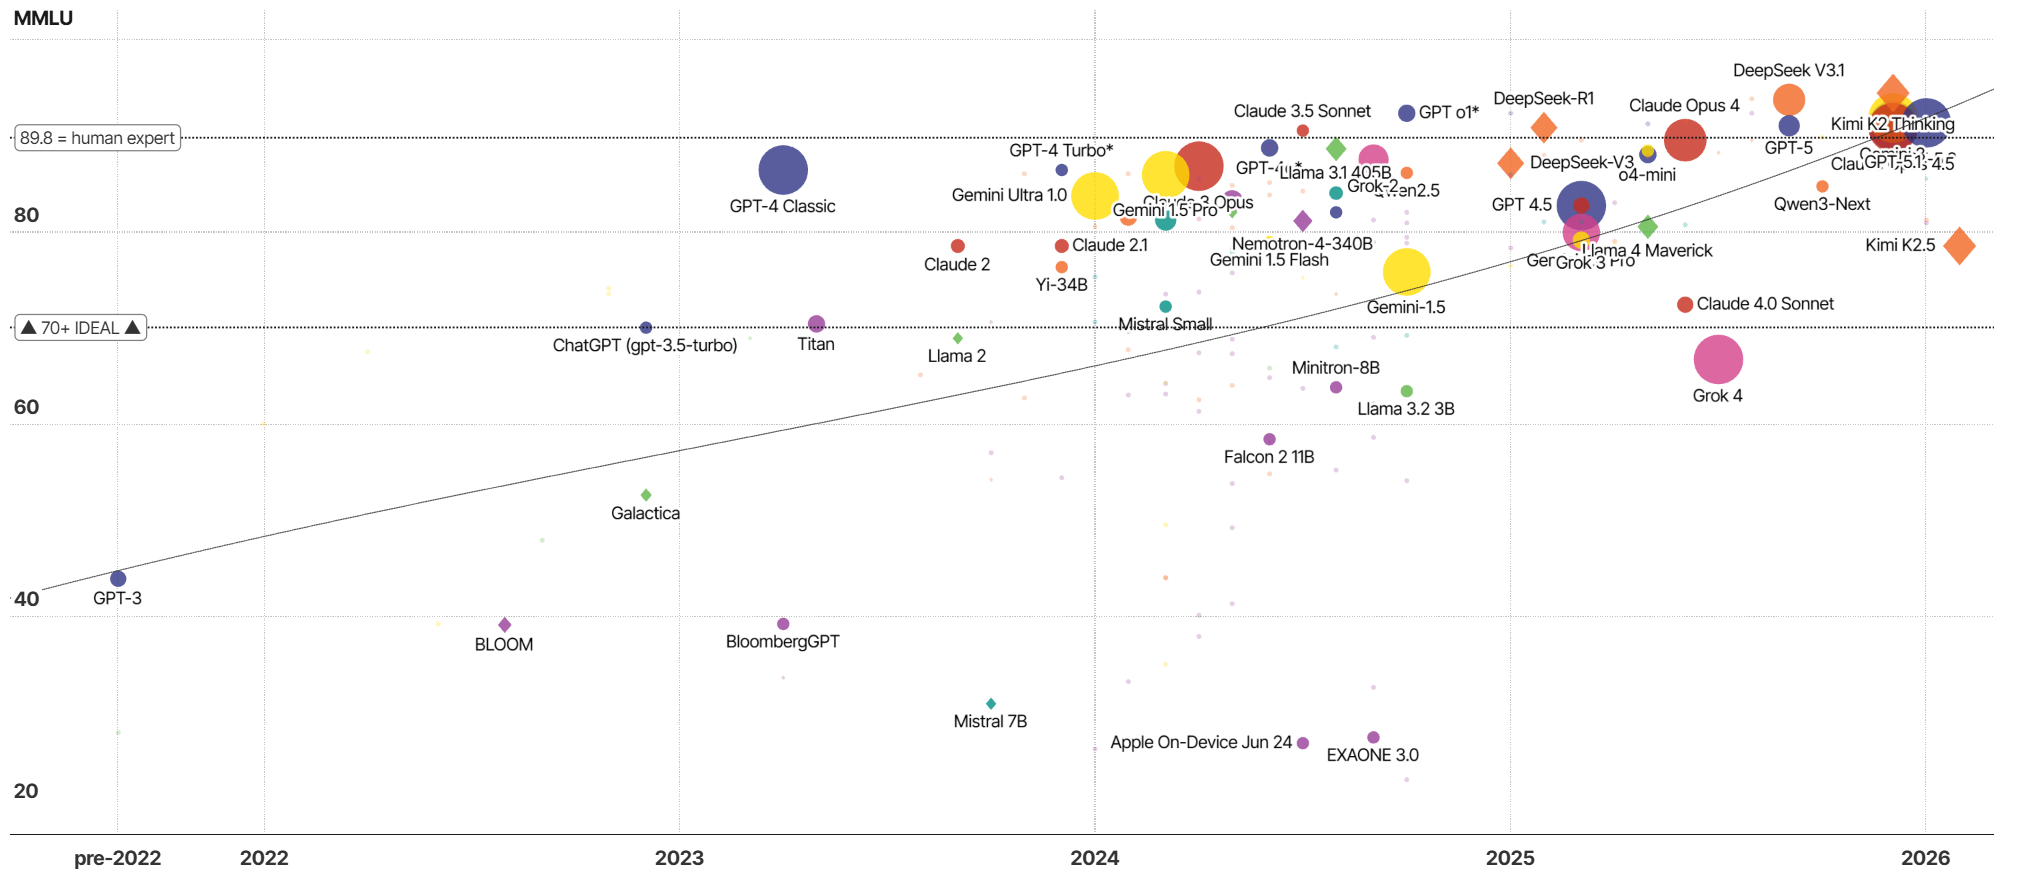
\includegraphics[width=0.9\linewidth]{image/llm_develop.png}
    \caption{主流大语言模型发展演进图source: LifeArchitect}
    \label{fig:llm}
\end{figure}

\subsection{AI模型量化技术}
在量化技术的演进历程中，早期的研究主要集中在将32位单精度浮点数FP32或16位半精度浮点数FP16/BF16压缩为INT8\cite{int8quant}。然而，大语言模型的激活值中普遍存在严重的离群值（Outliers）现象，这些长尾分布的离群值对模型的最终输出精度起着决定性作用。传统的整数统一量化（Uniform Quantization）\cite{int8quant}在面对这种高动态范围的数据时，往往会导致正常激活值的精度被严重挤压，进而引发模型困惑度（Perplexity）的急剧上升和准确率的崩溃。为此，学术界与工业界开始将目光转向低比特浮点数（Low-bit Floating Point）格式以及更加精细的块级微缩放（Block-wise Microscaling）技术。诸如开放计算项目（OCP）提出的MXFP8、MXFP6、MXFP4标准\cite{rouhani2023microscaling}，NVIDIA在Blackwell架构中引入的NVFP4\cite{nvidia2024nvfp4}格式，以及HUAWEI针对Acsend NPU架构优化的HiFloat8\cite{hifloat8}(HiF8) ,HiFloat4\cite{hifloat4}（HiF4）格式，均代表了当前量化数值格式的最高水平。这些格式通过在特定大小的数据块（Block或Group）内共享指数或缩放因子，成功在极低比特下保留了浮点数的动态范围优势，实现了极具竞争力的精度与性能提升之间的平衡。

\subsection{AI芯片算力规格演进}
数值精度格式的百花齐放与算法层面的混合精度（Mixed-Precision）演进，不可避免地与底层硬件张量核心（Tensor Core）或乘加运算阵列（MAC Array）的固定微架构产生了深刻的矛盾。现代商业AI加速器在设计计算处理单元（PE）时，通常采用固化的算力比例分配。例如，在NVIDIA的架构体系中，从Ampere\cite{nvidia2020ampere}到Blackwell\cite{nvidia2024blackwell}，其张量核心（Tensor Core）的稠密算力配比通常严格遵循物理位宽的反比关系，即在同样的硅片面积上，FP8的算力是BF16/FP16的两倍，而FP4/INT4的算力又是FP8/INT8的两倍，形成了经典的1:2:4算力配比。这种固定的硬件逻辑在面对未来大模型高度异构的混合精度量化和低比特精度压缩需求时，显得极其僵化。前沿的量化感知训练\cite{int8quant}（QAT）和训练后量化\cite{lin2024awq,frantar2022gptq}（PTQ）研究表明，大模型中只有极少数对精度极度敏感的层或通道需要保留在BF16或FP8的高精度格式，而高达80\%至90\%以上的权重和激活值可以被安全地压缩至FP8甚至更低的FP4精度。如果继续沿用传统的1:2:4算力配比架构，当系统仅需执行大量极低精度张量运算时，低精度的硬件算力受制高精度算力的面积占用无法实现指数级的增长，造成了算法与硬件需求的不匹配，以及硬件芯片面积和静态功耗的巨大浪费。
\begin{table}[htbp]
    \centering
    \caption{英伟达Tensor Core 算力与架构演进}
    \label{tab:nvidia_compute_evolution_transposed}
    % 使用 tabular* 撑满行宽，设定为 4 列 (1列指标 + 3列产品)
    \begin{tabular*}{\textwidth}{@{\extracolsep{\fill}}lcccc@{}}
        \toprule
        \textbf{规格参数} & \textbf{A100} & \textbf{H100 } & \textbf{B100} & \textbf{Vera Rubin}\\
        \midrule
        \textbf{发布时间} & 2020年5月 & 2022年3月 & 2024年3月 &2025年1月\\
        \textbf{Tensor Core} & Ampere & Hopper & Blackwell & Rubin\\
        \midrule
        \textbf{FP64} & 19.5 & 67 & 30$^*$ & 33$^*$\\
        \textbf{TF32} & 156 / 312 & 495 / 989 & 900 / 1800 &  2000/4000\\
        \textbf{FP16/BF16} & 312 / 624 & 989 / 1978 & 1800 / 3500 & 4000/8000\\
        \textbf{FP8} & - & 1979 / 3958 & 3500 / 7000 & 17500/35000\\
        \textbf{INT8} & 624 / 1248 & 1979 / 3958 & 3500 / 7000 & 250/500\\
        \textbf{FP4} & - & - & 7000 / 14000 & 35000/50000$^*$$^*$\\
        \textbf{INT4} & 1248 / 2496 & - & - & -\\
        \textbf{Computility Ration} & 1:2:4:8 & 1:2:4:- & 1:2:4:8& 1:2:8.75:17.5\\
        \bottomrule
    \end{tabular*}
    
    \vspace{0.5em}
    \begin{minipage}{\textwidth} 
        \footnotesize
        \textbf{说明：}\\
        1. 算力单位统一为 \textbf{TFLOPS} (浮点) 或 \textbf{TOPS} (整数)，数值格式均为 \textbf{Dense (稠密算力) / Sparse (2:4 结构化稀疏算力)}。\\
        2. \textbf{FP8/FP6 支持度}：Hopper 架构首次引入 FP8；Blackwell 架构则进一步在微架构层面原生支持了 FP6 以及更低精度的 FP4。\\
        3. \textbf{INT4 演替}：Ampere 架构曾原生提供 INT4 加速；但从 Hopper 架构起，底层算力资源全面向浮点格式倾斜，移除了原生的 INT4 Tensor Core 支持，Blackwell 架构开始支持 MXFP4、NVFP4 等多种超低比特浮点精度格式。\\
        4. \textbf{FP64 算力说明 ($^*$)}：Blackwell 架构（B100）为了优化芯片面积与能效，移除了硬件层面的原生 FP64 Tensor Core 单元。实际是通过软件模拟计算得出的，并非真实的硬件Tensor Core算力支持。\\
        5.  \textbf{Rubin 算力说明 ($^*$$^*$)} 根据公布数据，Vera Rubin超级芯片种包含2颗Rubin GPU，其NVFP4推理算力为50PFLOS，训练算力为35PFLOS，均为dense稠密算力。
    \end{minipage}
\end{table}
因此，跳出传统硬件设计中数值位宽与算力之间配比的窠臼，基于底层算法对不同数值精度（如MXFP4、NVFP4、HiF4）的真实需求与数据分布特性，反向驱动底层张量核心中处理单元（PE）的微架构重构，具有极高的科学研究价值。

本课题旨在提出一种面向未来的大模型量化软硬件协同设计方案。我们将在算法层面深入剖析不同低比特格式在模型困惑度、推理速度和显存占用等关键维度的优劣并以此为算法层面的依据。在硬件层面设计高度灵活、可复用的点积计算单元，通过“搭积木”的方式可以组合形成不同的算力配比，探索诸如1:2:6、1:2:8、1:4:8甚至0:4:8 等全新算力配比下的多精度融合微架构，并在功耗、面积、模型推理效果及硬件制造成本之间进行详尽的综合评估。本研究不仅能够为解决未来万亿参数大模型在端侧及云端的高效推理提供理论依据，也能够为下一代定制化人工智能加速芯片（AI ASIC）及可重构处理器的演进指明软硬件协同优化的新路径。


% 解决上面的需求，难点，问题的已有方法，研究创新方案
\section{国内外研究现状}
大语言模型的高效推理部署涉及从推理算法框架到模型量化压缩表示，再到推理服务集群底层芯片电路的设计与优化。近年来，随着大模型在各类垂直领域的快速落地，国内外顶尖研究机构和科技巨头在量化格式设计与底层硬件加速领域展开了激烈的角逐，并催生了大量极具价值的研究成果。
\subsection{新型数值格式研究现状}
\textbf{16位与32位混合精度格式}:早期的低精度研究主要集中在16位和改进的32位格式上，旨在通过牺牲一定的尾数精度来换取更大的动态范围。Google 推出的 BF16\cite{burgess2019bfloat16} (Bfloat16) 格式保留了与 FP32 相同的8位指数域，极大地简化了混合精度训练中的溢出问题。NVIDIA 在 Ampere 架构中引入了 TF32\cite{TF32} (TensorFloat-32)，采用19位格式（8位指数和10位尾数），作为 Tensor Cores 中 FP32 的无缝替代方案。在学术界，Agrawal 等人（2019）提出了 DLFloat\cite{agrawal2019dlfloat}，这是一种专为深度学习训练和推理设计的16位浮点格式，通过优化指数和尾数的位宽分配，进一步提升了计算效率与硬件资源的利用率。

\textbf{8位低比特量化的发展与国产化探索:}随着推理需求的激增，8位浮点（FP8）成为了新的行业标准。开放计算项目（OCP）推出了 MXFP8\cite{rouhani2023microscaling}格式，引入了块缩放（Block Scaling）概念，即多个元素共享一个微指数，从而在8位级别实现了更优的数值分布。在国内研究与国产硬件适配方面，Luo等人针对华为Ascend架构提出了 Ascend HiFloat8\cite{hifloat8}格式。该格式通过变成编码，使得低精度数值表达范围和数值表征细粒度之间取了折中，为国产 AI 算力底座提供了一种新的低精度浮点解决方案。

\textbf{面向大语言模型的极低比特量化:}对于千亿参数级别的 LLMs，8位量化仍不足以将模型完全加载至单卡显存中，因此研究焦点逐渐转向4位及以下的极低比特格式。Dettmers 等人提出的 NF4\cite{NF4} (NormalFloat 4) 是针对正态分布权重在信息论上最优的4位数据类型，已被广泛应用于 QLoRA 等微调技术中。Lee等人进一步演进了这一思想，提出了 AMXFP4\cite{lee2025amxfp4}。该格式将非对称设计与微缩放（Microscaling）技术相结合，优化了4位格式下LLM推理的激活异常值，显著提升了极低比特下的模型准确性。Lo等人（2024）探索了更为极致的 NxFP4\cite{NxFP4}（Nanoscaling Floating-Point），通过引入 NanoMantissa（纳米尾数）和自适应微指数技术，实现了对大型语言模型的直接转换压缩。工业界方面，NVIDIA 在 Blackwell 架构中正式引入了 NVFP4\cite{nvidia2024nvfp4}，通过块级别的缩放因子在硬件层面支持高效的4位浮点推理；同时，OCP 标准也向下延伸出了 MXFP6\cite{rouhani2023microscaling} 和 MXFP4\cite{rouhani2023microscaling}。与之相呼应，华为等国内厂商也在积极布局类似 HIF4\cite{hifloat4} 的极低精度格式，以打破算力与访存的壁垒。当前主流AI芯片中数值精度格式表达如表\ref{tab:data_formats_scaling}所示。
\begin{figure}[htbp]
    \centering
    % 第一个图片的 minipage
    \begin{minipage}[b]{0.48\linewidth}
        \centering
        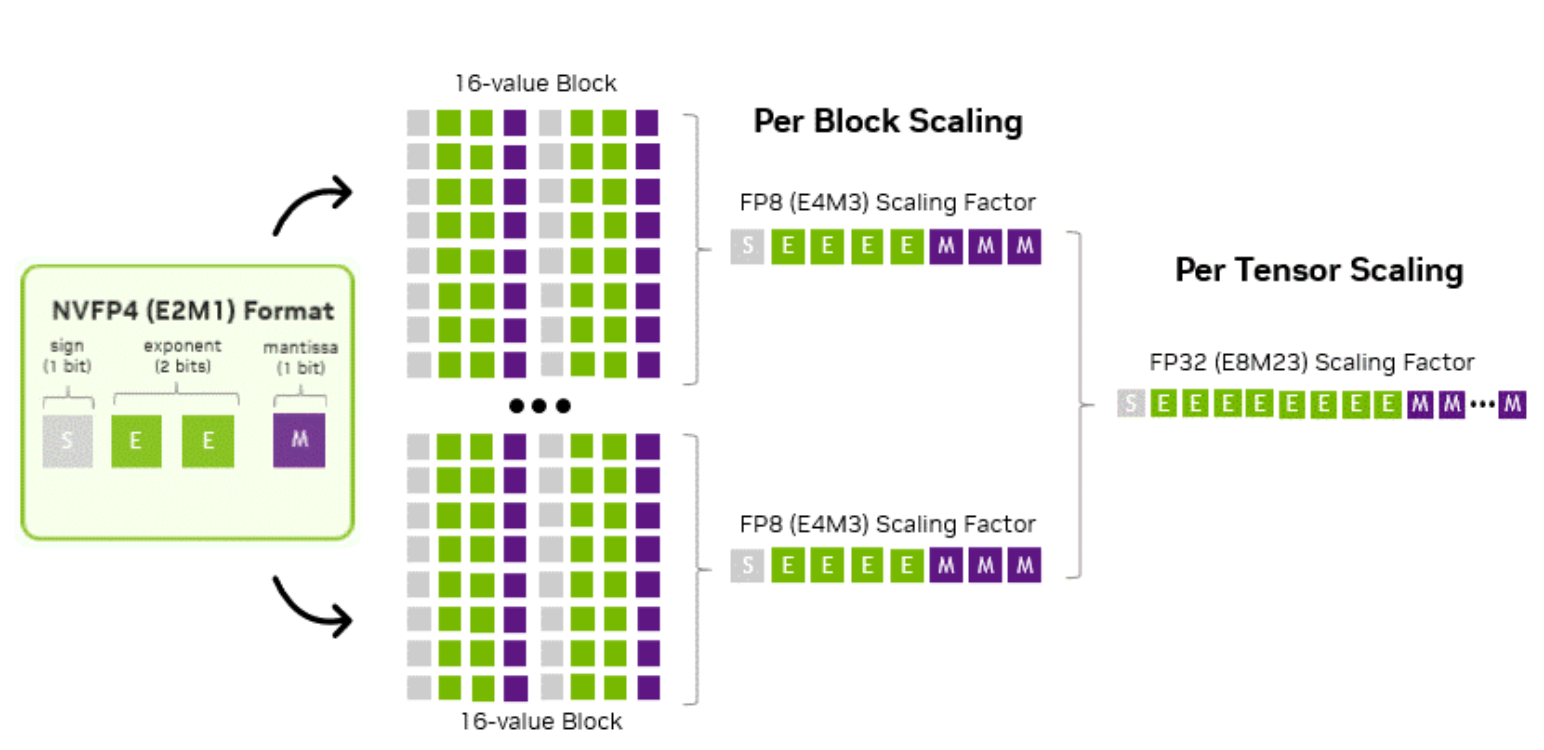
\includegraphics[width=\linewidth]{image/NVFP4.png}
        \caption{NVFP4两级缩放结构}
        \label{fig:NVFP4} % 建议改一个更清晰的label
    \end{minipage}
    \hfill % 在两个 minipage 之间添加弹性空白，让它们分别靠左和靠右对齐
    % 第二个图片的 minipage
    \begin{minipage}[b]{0.48\linewidth}
        \centering
        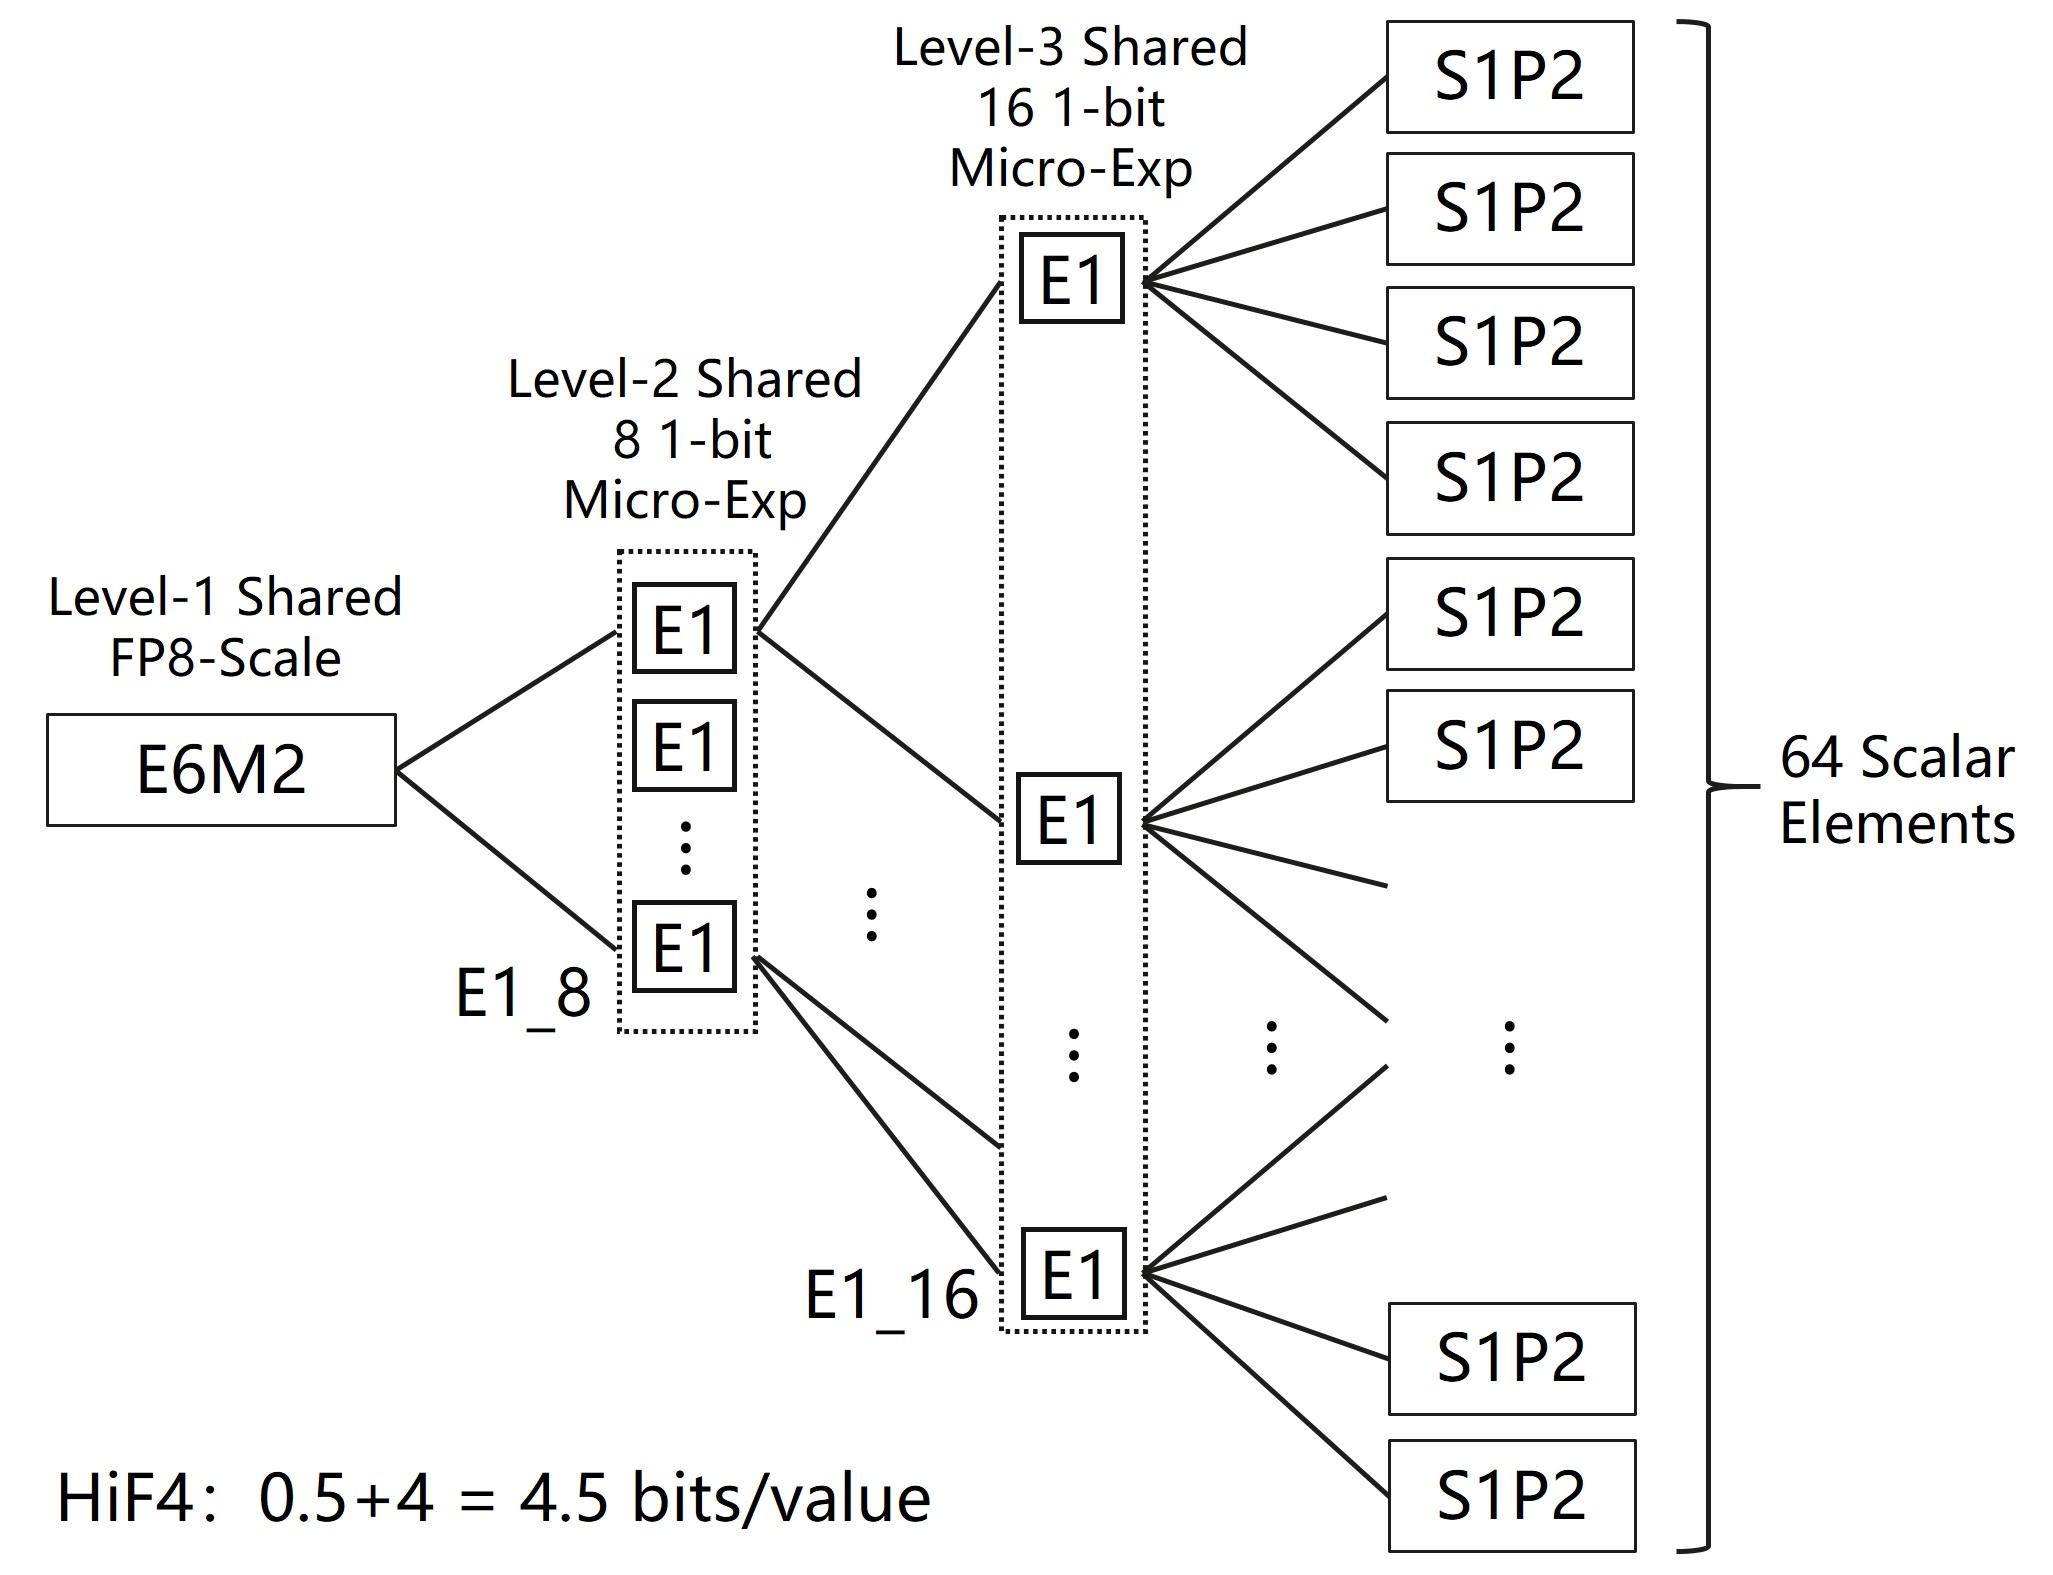
\includegraphics[width=\linewidth]{image/HIF4.png}
        \caption{HiF4 块浮点数格式结构}
        \label{fig:HIF4}
    \end{minipage}
\end{figure}
\subsection{模型量化算法发展}
随着大语言模型（LLM）参数规模的激增，模型量化成为降低显存占用和提升推理速度的核心技术，主要分为量化感知训练（QAT）和训练后量化（PTQ）两大路线：

\textbf{量化感知训练（QAT）：}通过在微调阶段前向传播中插入伪量化节点，让模型提前适应量化带来的截断误差。虽然 QAT 能够挑战极低比特（如 2-bit/3-bit）的极限精度，但由于需要计算梯度和更新权重，其计算成本对于千亿参数的 LLM 而言往往过于昂贵，因此QAT主要应用于端侧模型参数较小的模型量化中。

\textbf{训练后量化（PTQ）：} 由于大模型的重训代价极高，无需重新训练、仅依赖少量校准数据即可实现模型压缩的训练后量化（PTQ）逐渐成为主流研究范式。然而，LLM 激活值中普遍存在的极端异常值（Outliers）现象为量化带来了巨大挑战。针对该问题，近期研究主要从两个维度展开深入探索。在权重量化（Weight-Only）方面，Frantar等人提出了 GPTQ\cite{frantar2022gptq}，该方法巧妙利用二阶海森矩阵（Hessian）信息进行局部误差补偿，通过逐层量化并动态调整未量化权重，奠定了将大模型高效压缩至 4-bit 的基石。随后，Lin 等人提出了AWQ\cite{lin2024awq}，该研究发现并证实了并非所有权重同等重要；其通过分析激活数据精准识别出约 1\% 的“显著权重”，并实施硬件友好的缩放保护，在避免引入混合精度的前提下显著提升了量化性能。对于权重与激活双量化方案，Dettmers 等人开创性地提出了 LLM.int8\cite{LLMINT8}通过混合精度分解策略，在推理时将包含严重异常值的极少数通道剥离至 FP16 计算，其余通道量化为 INT8，成功实现了无损的 W8A8 推理。为进一步降低动态计算开销，Xiao 等人提出了 SmoothQuant\cite{xiao2023smoothquant}，引入一种数学等价变换策略，利用离线计算的平滑因子将激活值中剧烈波动的量化难度“转移”并分摊至权重端，实现了高效的静态 W8A8 量化。此外，为了向更极限的 W4A4 量化发起冲击，研究人员进一步提出了 SVDQuant\cite{li2024svdquant}，创造性地引入奇异值分解（SVD），通过提取高精度低秩（Low-Rank）分支来专门吸收激活异常值及极低比特带来的截断误差，在保障生成质量的同时大幅优化了推理延迟。
\begin{table}
    \centering
    \caption{深度学习数据格式与缩放因子特征}
    \label{tab:data_formats_scaling}
    
    % 采用 tabular* 环境，\textwidth 表示撑满当前文本行宽
    % @{\extracolsep{\fill}} 会自动计算并均匀分配列间距
    \begin{tabular*}{\textwidth}{@{\extracolsep{\fill}}lcccccc@{}}
        \toprule
        \textbf{格式} & \textbf{符号} & \textbf{指数} & \textbf{尾数/整数} & \textbf{Group} & \textbf{缩放因子} &\textbf{平均位宽} \\
        \midrule
        FP32 & 1 & 8 & 23 & - & - &32 \\
        TF32 & 1 & 8 & 10 & - & - &19 \\
        FP16 & 1 & 5 & 10 & - & - &16\\
        BF16 & 1 & 8 & 7  & - & - &16\\
        INT16 & 1 & 0 & 15 & - & - &16\\
        \midrule
        FP8 E4M3 & 1 & 4 & 3 & - & - &8\\
        FP8 E5M2 & 1 & 5 & 2 & - & - &8\\
        INT8 & 1 & - & 7 & - & -&8 \\
        \midrule
        FP6 E3M2 & 1 & 3 & 2 & - & - &6\\
        FP6 E2M3 & 1 & 2 & 3 & - & - &6\\
        FP4 E2M1 & 1 & 2 & 1 & - & - &4\\
        INT4 & 1 & - & 3 & - & - &4\\
        \midrule
        MXFP8 E4M3 & 1 & 4 & 3 & 32 & E8M0 &8.25\\
        MXFP8 E5M2 & 1 & 5 & 2 & 32 & E8M0 &8.25\\
        MXFP6 E3M2 & 1 & 3 & 2 & 32 & E8M0 &6.25\\
        MXFP6 E2M3 & 1 & 2 & 3 & 32 & E8M0 &6.25\\
        MXFP4 E2M1 & 1 & 2 & 1 & 32 & E8M0 &4.25\\
        \midrule
        NVFP4\textsuperscript{*} & 1 & 2 & 1 & 16 & FP8 E4M3 &4.5\\  
        HiF4\textsuperscript{\dag} & 1 & 2 & 1 & 64 & UE6M2\textsuperscript{**} &4.5\\
        \bottomrule
    \end{tabular*}
    
    \vspace{0.5em}
    % 使用与 \textwidth 等宽的 minipage 保证脚注左对齐且不会超出表格边缘
    \begin{minipage}{\textwidth} 
        \footnotesize
        \textsuperscript{*} \textbf{NVFP4}: 针对每个张量使用一个 FP32 缩放因子。\\
        \textsuperscript{**} \textbf{UE6M2}: 6位指数、2位小数，无符号位，指数偏移为48。\\
        \textsuperscript{\dag} \textbf{HiF4}: 内部还包含双重量化：第一级每4个元素共享一个E1指数，第二层每2个E1指数共享一个E1二级指数。
    \end{minipage}
\end{table}
\subsection{多精度资源复用型张量核心硬件架构研究}

与算法层面的格式创新相呼应，底层硬件微架构也在不断演进，以期最大化释放低精度计算的算力红利。从工业界主流计算产品来看，NVIDIA Tensor Core架构从Volta\cite{volta}架构支持FP16，到Ampere\cite{nvidia2020ampere}架构引入TF32和稀疏INT8支持，再到Hopper\cite{nvidia2022hopper}架构全面支持FP8，最终演进至Blackwell\cite{nvidia2024blackwell}架构原生支持FP16/BF16、FP8、FP6及NVFP4等全栈格式，严格维持了1:2:4的性能提升比例，其更多的也是从硬件设计层面进行资源复用,节省芯片面积的角度出发，实现多精度复用的张量计算单元设计。

在学术界，针对张量计算硬件架构设计中也意识到了资源复用的重要性，通过分析其硬件架构中面积和功耗占比较大的单元是乘法器，因此针对张量计算单元中乘法器的复用设计，主要形成了时间复用（Time-Multiplexing）与空间复用（Space-Multiplexing）两种主流硬件设计范式。

时间复用架构主要通过多周期的时间跨度来合成高精度计算。其核心思想是配置基础的低比特乘法单元，通过多次迭代低比特的乘积累加（MAC）操作，逐步生成高比特的计算结果。代表性工作如 Lee 等人提出的 UNPU\cite{unpu} 以及 Sharify 等人的 Loom\cite{loom}，它们利用位串行（Bit-serial）或动态子字处理机制，实现了从 1-bit 到 16-bit 权重的完全可变精度支持。尽管时间复用提供了极高的位宽灵活性与硬件极简性，但由于多次低比特计算会显著增加周期开销并严重限制系统吞吐量，在当前追求极致并行算力的张量核心设计中，较少被作为首选的主力方案。

相对而言，空间复用架构通过在单周期内对物理乘法器进行细粒度切割与重组，实现了多路低精度运算的高效并行，是目前最广泛采用的设计方向。在最经典的整数与基础浮点乘法器复用中，Sharma 等人提出的 Bit Fusion\cite{bitFUSION} 是极具代表性的奠基性工作。它巧妙利用了二维对角线移位累加结构，实现了低比特整数乘法器的动态物理拼接。而在乘法器切分层面，三星在ISSCC2022\cite{Samsung}上提出了一种高度优化的乘法器位分解策略。该架构将大乘法器的尾数部分拆解为 8x8、8x4 和 4x4 的基础阵列，通过配合移位器不仅支持了 12 位尾数的 FP16 计算，还能在完全相同的硬件逻辑下通过空间重构，单周期并行执行两路 INT8 或四路 INT4 的乘法运算，极大提升了面积利用率。
\begin{figure}[htbp]
    \centering
    % 第一个图片的 minipage
    \begin{minipage}[b]{0.48\linewidth}
        \centering
        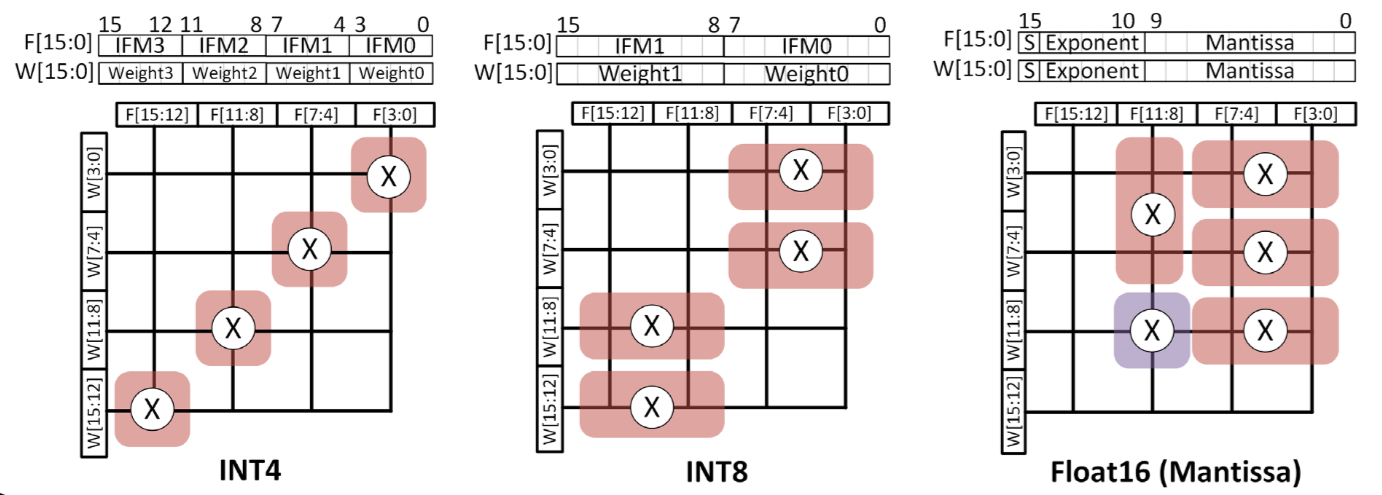
\includegraphics[width=\linewidth]{image/Samsung.png}
        \caption{细粒度乘法器分解复用}
        \label{fig:samsung-method}
    \end{minipage}
    \hfill % 在两个 minipage 之间添加弹性空白，让它们分别靠左和靠右对齐
    % 第二个图片的 minipage
    \begin{minipage}[b]{0.48\linewidth}
        \centering
        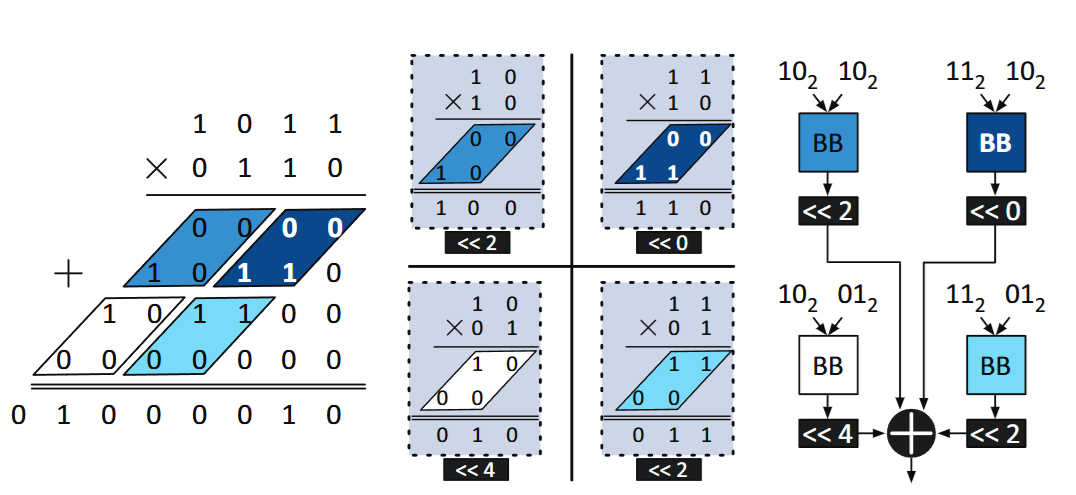
\includegraphics[width=\linewidth]{image/bitfusion.png}
    \caption{位融合乘法器分解复用}
    \label{fig:bitfusion}
    \end{minipage}
\end{figure}
随着微缩放格式（Microscaling, MX）和低精度浮点（如 FP8、FP6、FP4）在软硬协同量化中的兴起，空间复用设计正向着复杂数据类型演进。针对 MX 格式，Rouhani 等人的 MXDOTP\cite{mxdotp} 以及 ASAP\cite{asap} 加速器从 RISC-V 指令集扩展与非对称架构层面，实现了高效的微缩放浮点空间复用。在多精度融合计算方面，Fused FP8\cite{fusedFP8} 方案设计了共享块缩放因子的 4 路 FP8 点积与 FP32 累加的高效空间复用数据通路；而 MPICC\cite{mpicc} 则引入了支持随机舍入（Stochastic Rounding）的混合精度 MAC 单元，专为超低精度训练与推理优化。

针对非主流的新颖数值类型与软硬协同，面向大模型对异常值和激活分布的敏感性，底层硬件开始直接支持自适应的数据格式切换。DACAPO\cite{dacapo}、ANT\cite{ant} 以及 M-ANT\cite{mANT} 等工作深入探讨了如何在乘法器阵列内部重构自适应数值类型逻辑。这些设计允许张量核心根据算法层的分组量化策略，在不同精度组之间动态切换硬件组合方式，进一步提升了多精度复用架构对动态算法负载的亲和力。

\section{课题研究内容与方案}

虽然国内外在微缩放数值格式设计和特定用途处理单元微架构方面均取得了长足的进步，但在软硬协同优化的深度融合上仍存在明显的断层。算法研究者倾向于提出高度定制化的数值精度格式，但底层硬件若缺乏原生支持，往往只能回退至高精度格式进行计算。这不仅引入了额外的量化与反量化开销，也导致高精度算力的大量闲置。反之，硬件工程师为保证处理器的通用性，多采用保守的数值格式和刻板的 1:2:4 算力演进路线，难以有效适配新型微缩放格式的演进。

因此，本课题围绕“算法负载分析”与“硬件架构重构”双线展开，提出一种“自上而下需求剖析，自下而上架构重构”的闭环软硬件协同设计方法论，为算法的新型数值精度格式与硬件底层单元设计之间搭建起一个系统的桥梁，从而可以更好地推动未来算法和硬件协同发展，打造良好地正向循环。

整体研究方案划分为三个递进的核心层级：首先在算法层面构建以微缩放浮点格式为主的不同数值精度在开源LLM模型上的实验，配合主流模型量化算法探寻数值精度表达与模型推理速度、显存占用、模型准确度等因素之间的定量分析，从而为模型算法的量化数值精度选择提供模拟预估；其次在微架构层面设计支持细粒度资源复用的多精度点积单元（PE），并根据不同的参数配置生成多种类型的PE单元，并分析其面积、功耗、性能数据；最后在系统层面探索非传统算力配比下的点积单元构成，搭建一套综合硬件PPA与软件模型算法负载收益的架构探索仿真系统。

\subsection{数值精度格式对大模型推理的影响分析与建模}

如果缺少针对算法负载分析，那么硬件设计就无法与芯片应用场景收益闭环“，因此必须透彻理解各数值精度格式的数值表征特点及其在大模型算法应用时的具体收益。因此本研究将建立一套标准化的数值精度与模型推理效果评测实验，横向对比 BF16、MXFP8、MXFP6、INT8、MXFP4、NVFP4 以及 HiF4 格式在大语言模型推理中的具体表现。

各类低比特浮点格式的核心差异在于组粒度（Group Size）、共享缩放因子格式以及基本元素位宽的分配。在组粒度上，最新使用的整个张量共用一个缩放因子，从而使得整个张量的数据表征满足对应数据表达范围。之后，随着大模型算法的发展，逐渐出现逐token，逐channel以及更细粒度的分组量化范围。组粒度越小，量化过程中数据受到异常值的影响就越小，相应的量化误差也就越小，但是缺点是需要存储更多的缩放因子数据以及对硬件计算或反量化的计算要求也越高。因此实验中我们将探索常用的数据量化分组如32，64，128，256等，探索分组粒度与量化效果之间的关系。

在量化数据存储占用方面，我们可以分析量化为不同数值精度下平均的位宽占用。BF16/FP16为16bit。MXFP8为8.25bit。MXFP6为6.25bit。MXFP4为4.25bit。NVFP4约为4.5bit。HiF4为4.5bit。因此在可量化数据的模型存储，即线性层权重占用方面，4bit的超低精度格式内存占用减小到原来的28\%左右，8bit的低精度格式内存压缩约一半，缓解了模型的显存占用压力“存储墙”。同时，当前访存带宽在大模型推理训练中越来越重要，低精度的量化压缩缩放，也成倍缓解了通信访存的带宽开销，一定程度上缓解了系统的“通信墙”。

在模型效果评测实验上，首先一个共识是：“当前低精度数值精度主要应用在张量计算中（模型中的矩阵乘（GEMM/GEMV）运算）”。在大语言模型常见结构中，矩阵乘/矩阵向量乘主要是Attention中的Q K V和FFN（MoE）模块的计算，也就是需要针对模型的不同部署需求，合理选择该部分输入/中间激活值（左矩阵）和模型权重（右矩阵）的数据精度选择。
\begin{figure}[ htbp]
    \centering
    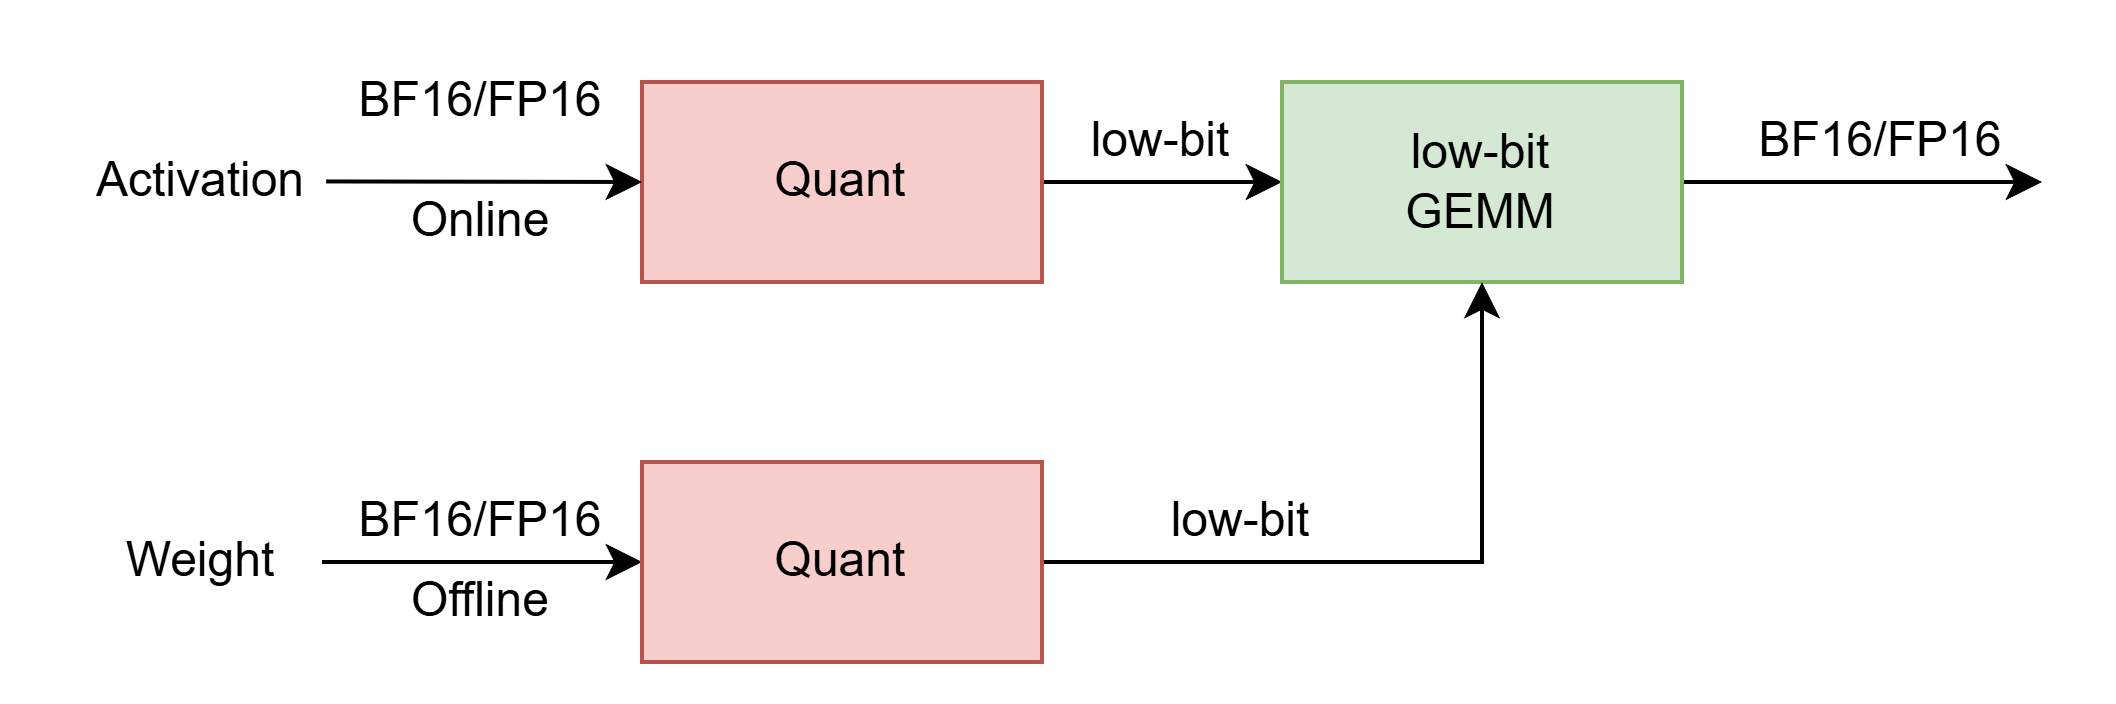
\includegraphics[width=0.55\linewidth]{image/Quant_compute1.png}
    \caption{硬件支持的低精度量化计算流程}
    \label{fig:quant_a}
\end{figure}
\begin{figure}[ htbp]
    \centering
    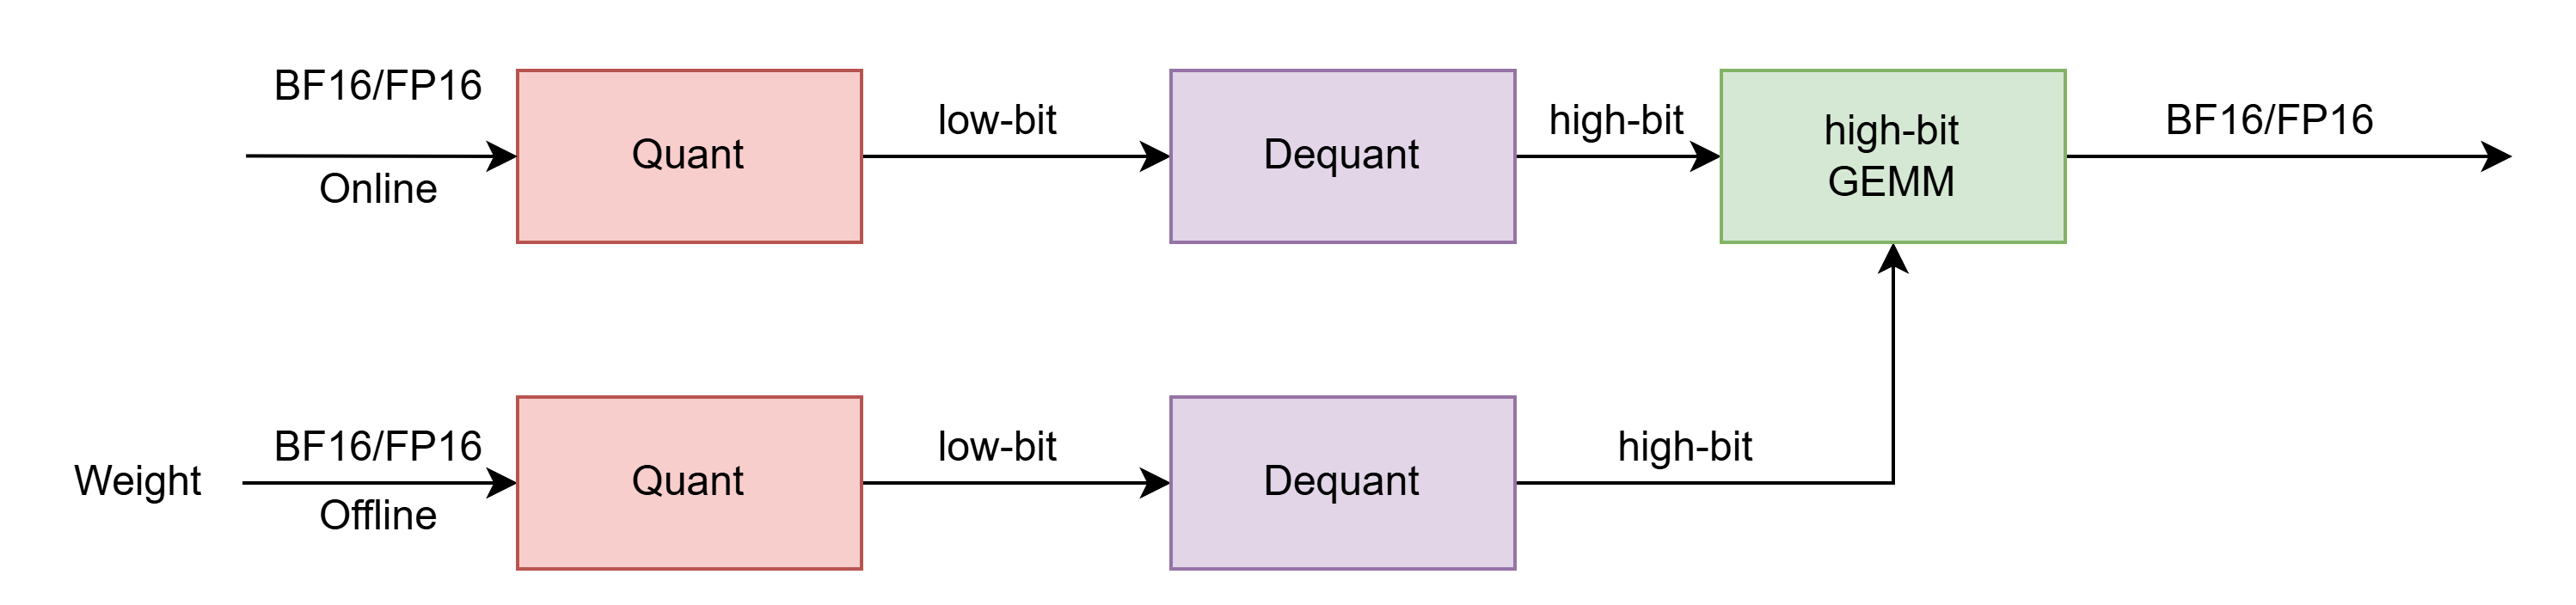
\includegraphics[width=0.75\linewidth]{image/Quant_compute2.png}
    \caption{硬件未支持的低精度量化计算流程}
    \label{fig:quant_b}
\end{figure}

在算法数值精度实验方案部分，首先可以根据模型的结构组成，计算模型的非线性层：线性层的计算负载，即对应芯片中vector计算与matrix计算的算力需求，为未来芯片设计规格提供设计参考。其次，主要完成测试大模型算法结构中的线性层接口的替换。针对硬件底层直接支持的数值精度计算，如\ref{fig:quant_a}和\ref{fig:quant_b}所示，离线完成权重参数的量化，在线性计算前将输入激活值量化，从而可以充分利用硬件的低精度张量计算。针对硬件尚未支持的数值精度，则需要将量化后的权重和激活值，在进行线性计算前反量化为硬件支持的高精度格式，模拟低精度数值格式量化的效果，再进行张量计算。


为验证理论模型的有效性，本研究将在当前主流的开源模型中进行部署评测，考虑到实验平台的成本，将选择20B以下的中小模型进行测试，以 BF16 作为无损推理的精度进行对照，系统性地记录并分析不同的数值精度量化，在模型困惑度（Perplexity, PPL）与准确率衰减方面的效果，使用在 WikiText2 数据集进行困惑度实验测试，并在 MMLU 等基准测试中记录零样本准确率（zero-shot）。

由于MXFP系列数值精度已在英伟达相关显卡上得到了支持，因此可以统一评测相同模型在不同数值精度下的模型运行效果，显存占用,以及量化评估不同格式以及量化方案在控制异常值（Outliers）上的不同效果。反之，实验也可以在相同显存占用/模型大小下，对比不同数值精度量化模型的推理效果和运行功耗信息。

\subsection{可复用多精度点积单元的微架构重构}

当前张量计算单元（Tensor core/cube）中，核心部分是将大的矩阵切分成更小的点积单元计算，通过合理的数据传输和状态调度，完成张量计算。因此本研究聚焦于底层核心的点积计算单元（PE）的架构设计，进而可以代表整个张量计算单元的数据。本研究将彻底摒弃了如\ref{fig:fma}中所示的传统依赖庞大全精度浮点乘加器FMA的设计范式，而使用多路点积单元DotProdcut的设计构成PE的基本设计，同时将针对新型数据结构提出一种更加细粒度，多层次，资源复用、支持多精度原生计算的新型点积微架构。
\begin{figure}[htbp]
    \centering
    % 左侧：FMA计算结构
    \begin{minipage}[c]{0.48\linewidth}
        \centering
        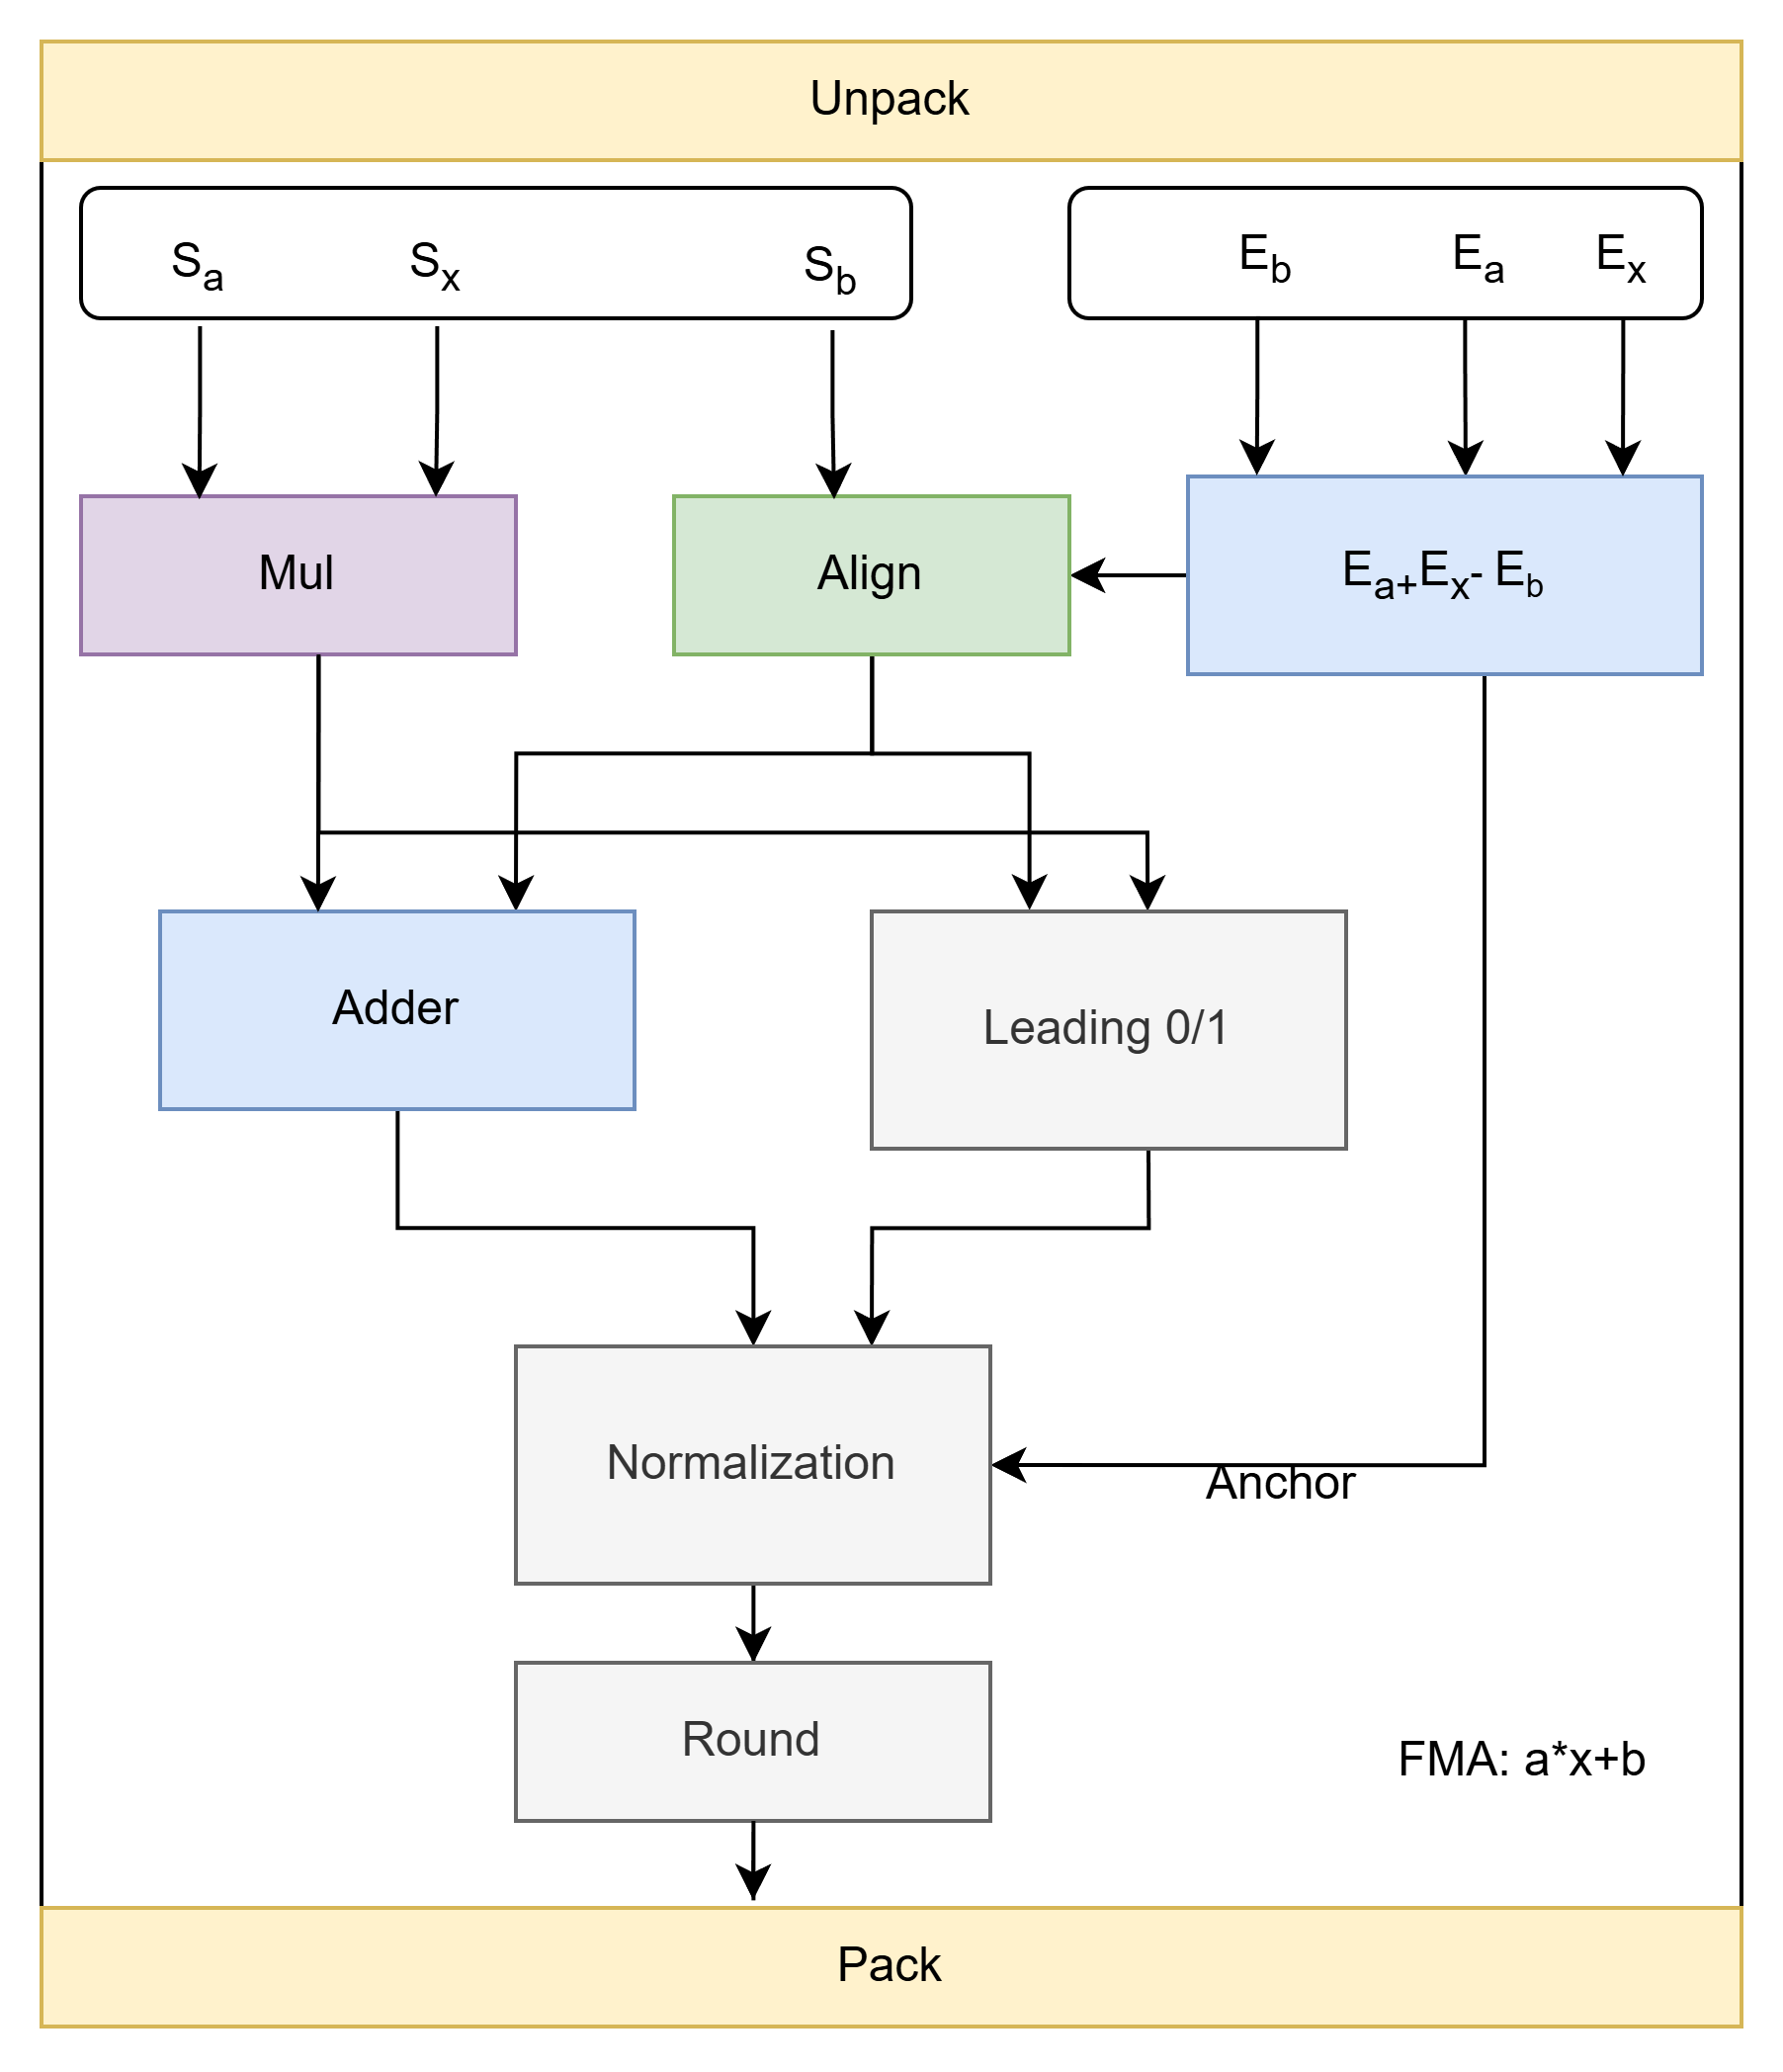
\includegraphics[width=\linewidth]{image/fma.png}
        \caption{FMA计算结构}
        \label{fig:fma}
    \end{minipage}
    \hfill
    % 右侧：点积单元结构构成
    \begin{minipage}[c]{0.4\linewidth}
        \centering
        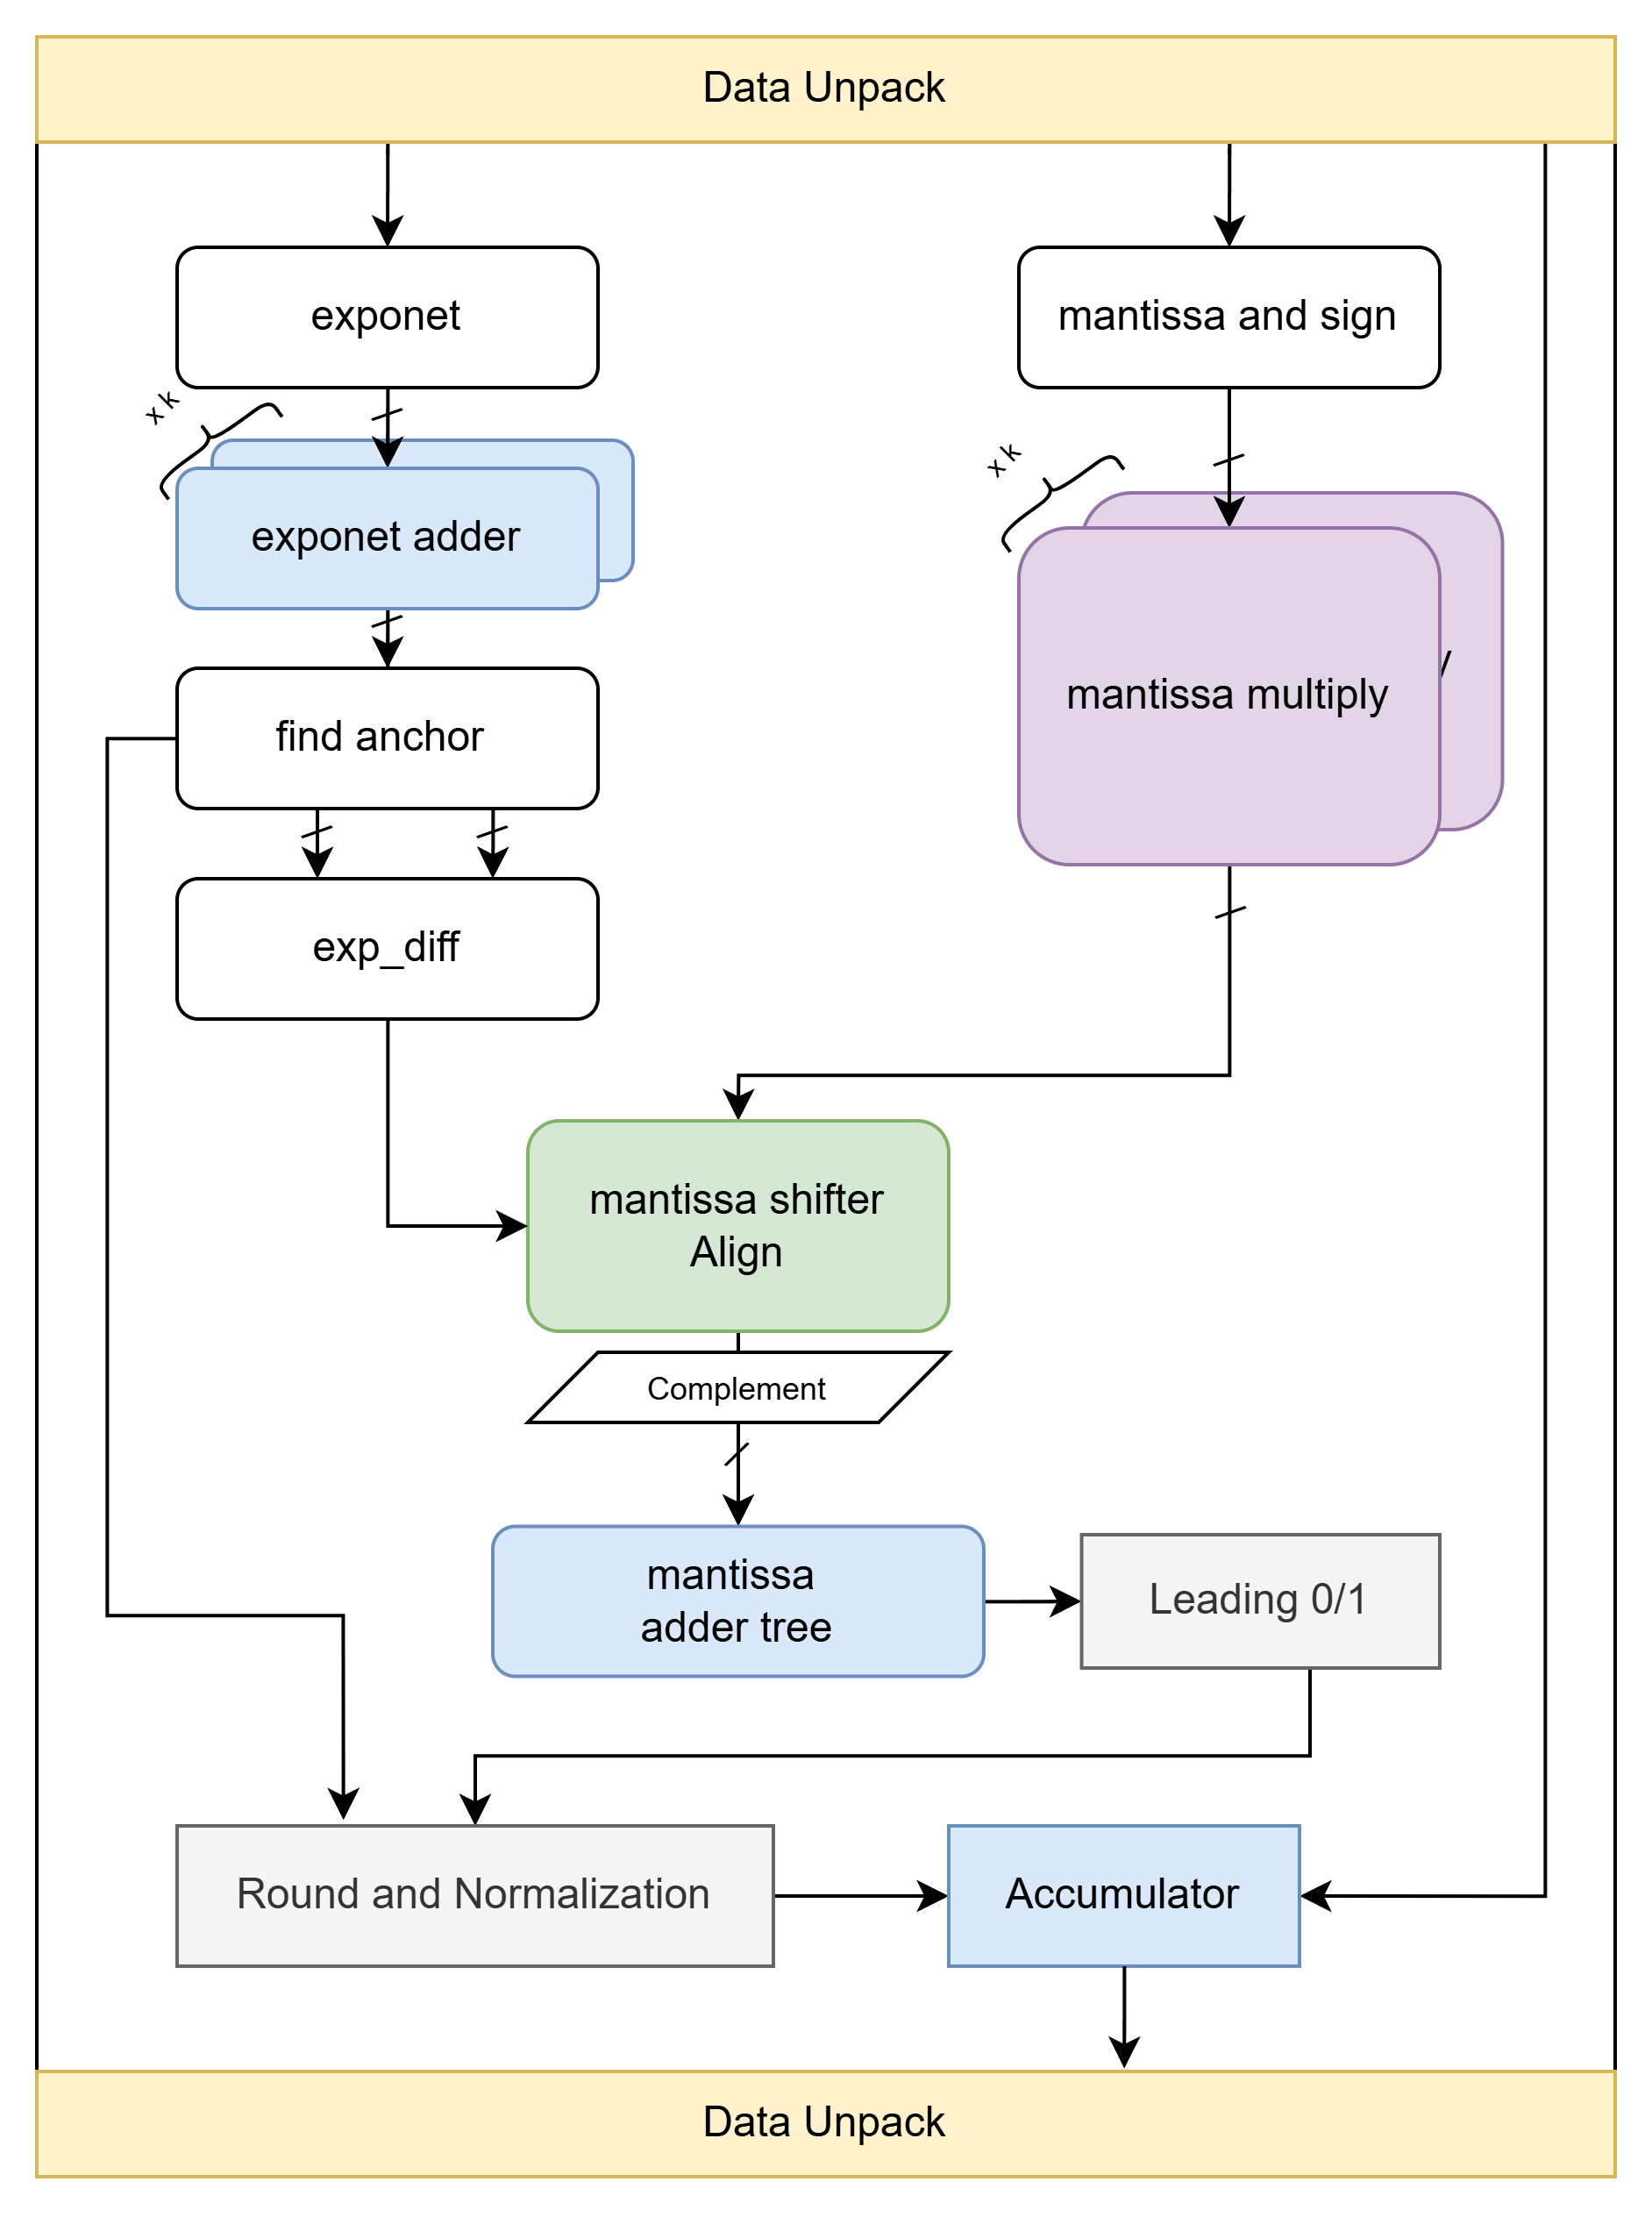
\includegraphics[width=\linewidth]{image/dot_product.png}
        \caption{点积单元结构构成}
        \label{fig:dotproduct} 
    \end{minipage}
\end{figure}
当前大多数支持多种精度张量计算加速的专用单元设计中，都会为了节省宝贵的芯片面积,而进行资源复用，即在重复利用相同数据通路/数据带宽下，在模块内部共享计算资源，实现支持不同精度格式的张量计算，而不是为每种数值精度格式设计独立的通路和计算单元，这也是维持传统的按位宽比例进行算力配比的主要原因。
因为芯片设计中面积的是一个重要的限制和约束条件，因此我们也将遵循计算资源复用的这一前提，节省芯片面积。为实现在同一硬件结构中对从 BF16 到MXFP4以及各类极低比特微缩放格式（NVFP4, MXFP4, HiF4 ）的兼容，本研究将瞄准高度模块化的可重构点积单元设计。其核心逻辑架构如\ref{fig:dotproduct}所示，重点优化路径如下：
\textbf{多格式数据解包与指数预处理：}在数据流入阶段，专用元数据解析单元，根据控制信号完成对输入数据的格式解包，分离输入数据中的符号位，指数，尾数，以及缩放因子。
针对微缩放格式，设计在解包阶段进行统一化处理，MXFP8(E5M2、E4M3）与MXFP6(E3M2、E2M3)均转为E5M3的标准格式，统一模块内部后续计算。针对MXFP4、NVFP4、HiF4,考虑到其极低的位宽，因此在解包阶段，将其两位指数融合到尾数部分，避免碎片化的指数加法与后期的移位对齐，同时可以引入基于查找表（LUT）的计算架构，实现输入两个4bit数据，即可查表获得浮点乘法结果，替代传统的高开销移位器和乘法器开销。

针对\textbf{指数加法}部分，所支持的数值格式中，主要包含8bit（BF16）与5bit(FP16、MXFP8/6)的无符号数加法，因此实现部分指数加法计算的复用。在\textbf{尾数乘法}部分，也是点积单元资源占用的主要部分，需要根据涉及的尾数位宽进行乘法器的资源复用。E2M1的格式定义，将指数融合到尾数后，4位位宽即可满足所以情况；MXFP8/6的尾数部分最大也是4bit位宽。此外BF16尾数位宽8位、FP16尾数位宽12位。因此仅需要支持多路的4bit、8bit、12bit的尾数乘法设计。当涉及FP16的12位尾数乘法时，可以采用8X8、8X4、4X4的乘法器组合，配合移位器实现1路12X12、2路8X8、4路4X4的无符号数尾数乘法。

点积单元与乘加融合FMA单元一个很大的区别，就是点积单元内部需要多路的浮点数指数对位，因此需要计算多路的指数加法、求最大值（对齐锚点），完成统一锚点下的尾数移位对齐，才能进行累加。在累加前，需要将尾数移位后结果转为有符号数，符号为两两解包的指数进行异或处理。在尾数加法树部分，也可以进行加法器的资源复用，设计的基本思想，就是多路的并行数值计算，在更低加法数层时，复用更高精度的加法器。即在传统的1：2：4配比下，FP4尾数首先进行一层两两加法计算，使得并行数据个数减半，与FP8的并行度一致，复用FP8的尾数加法器资源，同理，FP8的后续累加，可以复用更高精度的FP16/BF16尾数加法器资源。值得注意的是，针对多路的尾数加法树，需要权衡加法器位宽和点积计算精度。

尾数加法树之后，并行的数据统一转为了单个尾数计算数值，后续的浮点计算可以统一复用前导0检测、输入与规格化和累加器单元。这也是与多个FMA实现相同张量点积，可以节省的芯片面积。最后不断对上述高度模块化的流水进行深度优化：对指数加法、尾数乘法、加法树、前导零检测（LZD）、规格化及自适应舍入（Rounding）等关键模块，进行时序、面积与功耗的协同优化。

在上述资源复用的基本模块设计的指导思想下，我们可以改变单个点积PE单元支持的数值精度类型，从而可以得到BF16/FP16/FP8/FP4、FP8/FP4、以及支持单种数值精度BF16/FP16、FP8、FP4的PE单元设计。得到多种张量计算单元的“积木块”。在代码实现上，将采用敏捷的Chisel硬件开发语言完成多种参数配置下的新型点积单元PE单元设计，并使用综合工具评估其面积、功耗、时序性能，重点追踪激进架构下由多路选择网络和宽位累加树引入的面积惩罚及关键路径延迟，搭建一套从 RTL 到系统级的全栈验证综合环境。
% 在本研究提出的资源复用微架构指导下，计算单元（PE）已演变为一种高度模块化的“可配置积木”。通过改变单体 PE 支持的精度组合——涵盖从全兼容型（BF16/FP16/FP8/FP4）到特定精度型（如纯 FP4 或 FP8/FP4 组合，构建一个多维度的硬件设计空间。为实现高效的设计迭代，本研究采用敏捷硬件开发语言 Chisel 对不同参数配置下的 PE 进行 RTL 级重构。利用工业级 EDA 综合工具链，重点追踪在不同算力配比下，由复杂多路选择网络及高位宽累加树所引入的面积惩罚与关键路径时延波动。基于底层 RTL 真实反馈的 PPA（面积、功耗、时延）数据，为宏观架构的算力配比探索提供了坚实的物理层依据。
\subsection{灵活算力配比的深度探索与 PPA 综合权衡}

在此基础上，本研究旨在构建一个耦合算法收益与硬件代价的深度评价系统，探究软硬件参数间的非线性映射关系。算法层面的需求——包括但不限于模型困惑度（Perplexity）、推理准确度、内存带宽占用及TTFT等指标——与底层硬件的算力分布存在深刻的相互作用。结合前期在算法端开展的多精度量化实验，本研究将量化模型推理产生的精度收益曲线与硬件侧不同算力配比的 PPA 代价函数进行关联，从而对“算力分布 vs. 精度损失”这一核心矛盾进行敏感度分析。通过对比 1:2:4、1:2:8 乃至更激进的非对称配比方案，旨在寻找在特定模型规模与任务约束下的硬件配置最优解。

最终，本研究将通过软硬件协同设计，构建起“算法特性-精度分布-硬件架构-PPA成本”的闭环反馈仿真系统。不仅能论证激进算力配比方案的可行性，更能揭示大模型推理场景下软硬件协同设计的深度边界，为未来 AI 芯片设计中如何平衡算法的灵活性与硬件的极致能效提供系统性的理论指导。

\section{论文工作的总体安排}
论文工作将按照以下时间节点稳步推进：
\begin{itemize}
    \item \textbf{2025年09月 - 2026年03月}：完成开题报告，梳理国内外文献，确定具体研究方案。
    \item \textbf{2026年4月 - 2026年05月}：完成算法层面的量化、数值精度比较实验。
    \item \textbf{2026年5月 - 2026年6月}：完成PE 单元的微架构设计与 RTL 实现。
    \item \textbf{2026年7月 - 2026年08月}： 功能验证及 PPA 综合评估。
    \item \textbf{2026年09月 - 2026年12月}：搭建评价分析系统，整合软硬件协同系统设计，完成系统级仿真，整理实验数据。
    \item \textbf{2027年01月 - 2027年04月}：撰写毕业论文，准备预答辩与正式答辩。
\end{itemize}

\section{预期目标}
\begin{itemize}
    \item 完成常见开源模型在不同量化算法与数值精度格式下的性能分析实验，量化算法的工作负载与需求定义。
    \item 完成多精度资源复用型点积单元PE架构设计与 RTL 实现，获取多种参数配置下的PE单元PPA数据。
    \item 搭建软硬件分析仿真，基于算法负载的不同要求，整合探索硬件的各精度配比下的PPA数据，搭建软硬件收益分析系统。
    \item 通过软硬件协同的分析系统，希望可以对未未来软件算法量化数值精度选择与芯片厂商硬件下一代ai芯片算力配比与数值精度支持提供参考。
\end{itemize}







% ==================== 参考文献列表 ====================
\newpage 
\section{参考文献}
\begingroup
    \zihao{5} 
    \setlength{\bibsep}{0pt} 
    % 使用标准的按引用顺序排版的样式，或者使用 IEEEtran
    \bibliographystyle{unsrt} 
    \bibliography{ref} 
\endgroup


% \newpage
\vspace {10mm}
% % \begin{multicols}{1}
% \noindent {\zihao{5}\bf{附录X}.}

% {\zihao{5-}\setlength\parindent{2em}
% \textbf{附录内容}置于此处，字体为小5号宋体。附录内容包括：\textbf{详细的定理证明、公式推导、原始数据}等}

% % \end{multicols}

\end{document}